\subsection{Studienplanung: Was alles schief gehen kann-
  Leidensbericht eines Fünftsemesters}
Nun haben wir euch ja schon eine ganze Menge über die großen
Freiheiten bei der Studienplanung erzählt, sowie sogar noch einen
alternativen Plan vorgelegt. Nun fragt sich sicherlich der Eine oder
Andere, warum es nun noch mehr Text sein muss. Nun, wir dachten uns,
dass Planung gut und schön ist, aber nicht immer klappen muss. Also
dachten wir uns, dass wir am Beispiel eines mäßig begabten Studenten
das mal exemplarisch vorführen, inklusive angepassten Studienplans. So
sollt ihr aus seinen Fehlern lernen, was man nicht machen sollte, aber
auch, wie man eigene Fehler noch korrigieren kann. Dazu schreiben wir
jedes Semester, was der Student vorhatte und was es dann geworden ist...

\paragraph{Prolog}
Als ich anfing, hat uns die Fachgruppe neben der 1-ten uns
insbesondere ihren alternativen Musterstudienplan auf Seite 
\pageref{studienplan_neu}
ans Herz gelegt und
so nahm ich mir denn vor, brav danach zu gehen, aber alles kam ganz
anders...
\paragraph{Erstes Semester}
Geplant:
\begin{itemize}
\item Programmieren 1 - 6 Credits
\item Algorithmen und Datenstrukturen - 8 Credits
\item Diskrete Mathematik - 5 Credits 
\item Lineare Algebra - 10 Credits
\item Theoretische Informatik 1 - 5 Credits
\item Wissenschaftliches Arbeiten - 2 Credits
\item Summe: 36 Credits
\end{itemize}
Die Planung ging schon schnell nicht mehr auf, da ich noch damit
überfordet war, alle Hausaufgaben rechtzeitig und selbstständig zu
ersetzen. Insbesondere für Theoretische Informatik 1 war ich zu
unmotiviert und faul, und habe es dann nach den Weihnachtsferien
gekickt. Ich war dabei der Einzige der 5-6 Leute aus meinen Jahrgang,
die der Fachgruppenempfehlung gefolgt waren, alle anderen haben es
erfolgreich durchgezogen. Ich war also erst einmal gefrustet, vor
allem weil es für das Hören eines anderen Faches auch zu spät
war. Somit blieb alles beim offiziellen Musterstudienplan wie auf
Seite \pageref{musterstudienplan}:\\
Geschafft:
\begin{itemize}
\item Programmieren 1 - 6 Credits
\item Algorithmen und Datenstrukturen - 8 Credits
\item Diskrete Mathematik - 5 Credits 
\item Lineare Algebra - 10 Credits
%\item Theoretische Informatik 1 - 5 Credits
\item Wissenschaftliches Arbeiten - 2 Credits
\item Summe: 31 Credits
\end{itemize}

\paragraph{2. Semester}
Da mein Plan mit Theoretische Informatik 2 nicht aufging, musste ich
mir etwas anderes überlegen. Ich war nicht der Einzige und auf der
übrigens sehr empfehlenswerten Seite \url{http://www.clevershit.de/}
fragte jemand nach möglichen Fächern. Wir erfuhren, dass Technische
Informatik 2 trotz des Namens mit etwas Fleiß auch ohne Technische
Informatik 1 als Vorkenntnisse zu schaffen ist. Außerdem wollte ich
nach offiziellen Studienplan ein Mathewahlpflichtfach belegen. Zur
Auswahl standen Stochastik und Algebra. Ich entschied mich für
Stochastik. Dann habe ich  noch kurzfristig eine
Schlüsselqualifikation belegt, und zwar den Kurs ,,Einführung in die
wissenschaftliche Textverarbeitung mit \LaTeX\ '' \footnote{Der
  Anwendung verdankt ihr diesen Text ;)}.\newpage Geplant waren damit:
%das Ergebnis war dann folgende Planung:
\begin{itemize}
\item Programmieren 2 - 6 Credits
\item Technische Informatik 2 - 4 Credits
\item Logik  - 5 Credits 
\item Computernetze - 5 Credits
\item Analysis - 10 Credits
%\item Theoretische Informatik 1 - 5 Credits
\item Stochastik - 5 Credits
\item \LaTeX\ - 3 Credits
\item Summe: 38 Credits
\end{itemize}
Allerdings ging auch das nicht auf: Ich hatte in Technische Informatik
2 in der Tat keine Probleme der Vorlesung zu folgen, wenn ich denn mal
da war. Die Hausaufgaben für Stochastik, Programmieren 2, sowie Logik
forderten ihren Tribut und mein Vorlesungsbesuch wurde immer
sporadischer. Entsprechend bin ich dann durch die Prüfung
durchgefallen. Außerdem wollte ich eine gute Note in Analysis, da die
Gewichtung dort sehr stark ist. Entsprechend habe ich mich dann noch
von Programmieren 2 abgemeldet und übrig blieb folgendes:
\begin{itemize}
%\item Programmieren 2 - 6 Credits
%\item Technische Informatik 2 - 4 Credits
\item Logik  - 5 Credits 
\item Computernetze - 5 Credits
\item Analysis - 10 Credits
%\item Theoretische Informatik 1 - 5 Credits
\item Stochastik - 5 Credits
\item \LaTeX\ - 3 Credits
\item Summe: 28 Credits
\end{itemize}

\paragraph*{Drittes Semester}
Im dritten Semester musste ich nun also Theoretische Informatik 1 noch
einmal hören. Damals galt für mich noch die alte
Prüfungsordnung, sodass ich auch  Hardware-Software-Systeme
belegen musste. Außerdem musste ich ja noch die Klausur in Technische
Informatik 2 schreiben, weil ich diese ja (siehe oben) durch meine
Faulheit versemmelt hatte. Zudem musste ich mit den Nebenfach
anfangen. Ich entschied mich für Psychologie. Im
Schlüsselqualifikationsbereich fehlten mir nur noch 5 Credits. Da mir
eine Mitbewohnerin 
schon von der Vorlesung ,,Geschichte der Mathematik''  erzählt hatte,
und diese genau 5 Credits brachte ergab sich dann geplant:
\begin{itemize}
%\item Programmieren 2 - 6 Credits
\item Technische Informatik 1 - 4 Credits
\item Technische Informatik 2 - 4 Credits
\item Relationale Datenbanken 1 - 5 Credits 
\item Hardware-Software-Systeme - 5 Credits
\item Betriebssysteme - 5 Credits
\item Softwaretechnik 1 - 4 Credits
\item Theoretische Informatik 1 - 5 Credits
%\item Stochastik - 5 Credits
\item Einführung in die Psychologie - 5 Credits \footnote{Dies ist
    allerdings geraten, da zum Modul noch zwei andere Prüfungen
    gehören. Die drei ergeben zusammen 10.}
\item Geschichte der Mathematik- 5 Credits
\item Summe: 42 Credits
\end{itemize}
Natürlich kam es auch hier ganz anders als gedacht: Theoretische
Informatik 1 lief deutlich besser als erwartet, da doch noch
erstaunlich viel vom 1. Semester in Erinnerung geblieben war. Dafür
lief Technische Informati 1 gar nicht. Spätestens, als unserer
Professor in Relationale Datenbanken, Herr Balke, uns vom
SQL-Praktikum erzählte, dass einen 4 Credits im Wahlpflichtbereich
Informatik einbringt, war mir klar, dass ich dafür Technische
Informatik 1 sausen lassen würde. Aus ähnlichen Gründen scheiterte
Betriebssysteme: Zwei Tage später musste ich Theoretische Informatik 1
schreiben und wieder zwei Tage später Relationale Datenbanken 1. Also
meldete ich mich von Betriebssysteme ab und hoffte so genug Zeit für
die anderen Prüfungen zu haben. Bei Theoretische Informatik 1 klappte
es, bei Datenbanken und Psycholgoie nicht. Dafür habe ich Technische Informatik 2 im
2. Versuch bestanden und somit blieb es bei folgenden Geschafften:
\begin{itemize}
%\item Programmieren 2 - 6 Credits
%\item Technische Informatik 1 - 4 Credits
\item Technische Informatik 2 - 4 Credits
%\item Relationale Datenbanken 1 - 5 Credits 
\item SQL-Praktikum - 5 Credits
\item Hardware-Software-Systeme - 5 Credits
%\item Betriebssysteme - 5 Credits
\item Softwaretechnik 1 - 4 Credits
\item Theoretische Informatik 1 - 5 Credits
\item Geschichte der Mathematik- 5 Credits
\item Summe: 28 Credits
\end{itemize}

\paragraph{Viertes Semester}
So brach nun das vierte Semester an und somit das
Softwarentwicklungspraktikum (SEP). Nun freute ich mich darüber, schon
Computernetze und Technische Informatik 2 gemacht zu haben, blieb doch
als Pflichtfach nur Theoretische Informatik 2, und dazu noch zwei
Fächer aus der Psychologie, die den Rest des im WS angefangenen Moduls
bilden würden. Dazu kamen noch die Wahlmodule. Ich entschied
mich für Netzwerkalgorithmen, da ich Algorithmen und Datenstrukturen
vom 1. Semester noch in guter Erinnerung hatte. Aufgrund ähnlicher
Erfahrungen mit Hardware-Software-Systeme belegte ich außerdem die
Fortführung ,,Chip- und Systementwurf 1''.  Auch wollte ich endlich
die Klausuren für ,,Betriebssysteme'' und ,,Programmieren 2'', sowie
,,Relationale Datenbanken 1''
nachholen. Damit ergab sich dann folgende Planung:
\begin{itemize}
 \item Programmieren 2 - 6 Credits
 \item Betriebssysteme - 5 Credits
\item Relationale Datenbanken - 5 Credits
\item SEP - 8 Credits
\item Theoretische Informatik 2 - 6 Credits
\item Chip- und Systementwurf 1 - 4 Credits \footnote{Für den 1. Teil,
    also die Vorlesung plus Prüfung, der 2. Teil folgt im 5. Semester.}
\item Netzwerkalgorithmen       - 5 Credits
%\item Stochastik - 5 Credits
\item Der Mensch im sozialen Kontext/Das Individuum in seiner Entwicklung - 5 Credits \footnote{Wieder geraten da der 2. Teil
    des im 3. Semester angefangenen Moduls, beide ergeben zusammen 10}
%item Geschichte der Mathematik- 5 Credits
\item Summe: 44  Credits
\end{itemize}
Mein Plan war also diesmal deutlich reduzierter, da ja ganze 16 Credits
erst zur Prüfungsphase relevant wurden. So dachte ich und so täuschte
ich mich. Das SEP erwies sich in der Tat als so zeitaufwendig und
stressig, wie höhere Semester immer berichtet hatten. Mit Müh und Not
schaffte ich daneben die Zulassung für Netzwerkalgorithmen und
Theoretische Informatik 2. Da ich insbesondere bei letzten Fach nicht
das Gefühl hatte, groß etwas verstanden zu haben, habe ich die Prüfung
dann lieber geschmissen und aufs 6. Semester vertagt. Dafür lief das
SEP und die ,,Altlasten'' unter den Prüfungen deutlich besser: Der
Betreuer war sehr angetan von unserer Arbeit und ich konnte endlich
ein Häkchen hinter Betriebssysteme, Programmieren und Datenbanken
setzen. Offen blieben hingegen noch Chip- und Systementwurf, sowie das
große Psychologiemodul. Bei Chipentwurf fehlte mir noch das Praktikum,
da dies erst nach der Prüfung im 5. Semester fehlen würde. Und in
Psychologie würde ich den 1. Teil als Letztes im 5. schreiben, da ich
dort ja durchgefallen war und die nächste Prüfung erst wieder im
Wintersemester angeboten würde:
\begin{itemize}
%\item Programmieren 2 - 6 Credits
%\item Technische Informatik 1 - 4 Credits
%item Technische Informatik 2 - 4 Credits
%item Relationale Datenbanken 1 - 5 Credits 
%item SQL-Praktikum - 5 Credits
%
%\item Betriebssysteme - 5 Credits
 \item Programmieren 2 - 6 Credits
 \item Betriebssysteme - 5 Credits
\item Relationale Datenbanken - 5 Credits
\item SEP - 8 Credits
%\item Theoretische Informatik 2 - 6 Credits
%TODO: Anpassen nach CuSE Prüfung
%\item Chip- und Systementwurf 1 - 4 Credits \footnote{Für den 1. Teil,
%    also die Vorlesung plus Prüfung, der 2. Teil folgt im 5. Semester.}
\item Netzwerkalgorithmen       - 5 Credits
%\item Stochastik - 5 Credits
%TODO
%\item Psycholgoie - 5 Credits \footnote{Wieder geraten da der 2. Teil
%   des im 3. Semester angefangenen Moduls}
%item Geschichte der Mathematik- 5 Credits
\item Summe: 29  Credits
\end{itemize}

\paragraph{Fünftes und sechstes Semester}
Mittlerweile bin ich im fünften Semester und obwohl ich
schon einiges geschafft habe, bleibt auch noch einiges zu tun. Ich
muss endlich Technische Informatik 1, sowie meine versemmelte Psycholgieklausur nachholen. Außerdem fehlt mir
noch das 2. Mathe-Wahlpflichtmodul (ich entscheide mich für Numerik), sowie  das Praktikum für Chip-
und Systementwurf 1. Im Psychologie fehlt mir dann noch das Modul ,,Gesetzmäßigkeiten von Verhalten und mentalen Prozessen'':
\begin{itemize}
\item Technische Informatik 1 - 4 Credits
\item Seminar - 5 Credits
\item Teamprojekt - 5 Credits
\item Numerik - 5 Credits
\item Praktikum zum Chipentwurf - 6 Credits
\item Gesetzmäßigkeiten von Verhalten und mentalen Prozessen - 6
  Credits
\item Einführung in die Gebiete der Psychologie - 5 Credits (bereits
  im 3. Semester gehört, damals aber durchgefallen)
%\item SEP - 8 Credits
\item Summe: 36 Credits
\item Dazu kommen noch die 4 Credits des ersten Teils vom Chipentwurf
 sowie die 5 Credits aus den Psycholgievorlesungen im 4. Semester,
 also insgesamt 45 Credits.
\end{itemize}
Wenn alles nach Plan klappt, habe ich im 6 Semester also nur noch 21
Credits zu absolvieren, nämlich 6 für Theoretische Informatik 2, sowie
15 Credits für die Bachelorarbeit. Da ich in der theoretischen
Informatik starke Defizite habe, werde ich die Vorlesung wohl nochmal
hören. Meine Erfahrung sagt mir aber, dass wohl auch diese Planung
wieder nicht ganz hinhauen wird. Andererseits ist man flexibel und es
ist ja nicht das erste Mal, dass ich Fächer in Studienplan hin und her
schiebe und somit aus einer blöden Situation noch das beste raus
hole. Den sich daraus ergebenden Studienplan sieht ihr auf der
nächsten Seite. 
Bei den Credits habe ich eurer Modulhandbuch, soweit bekannt,
zugrunde gelegt, dennoch sind alle Angaben erstmal unverbindlich und
ohne Gewähr. Auch sind meine Angaben beim Nebenfach und den
Wahlfächern natürlich die, die ich belegt habe und somit natürlich nur
ein Vorschlag.
\paragraph{Nachbemerkungen}
Diese Geschichte ist mir wirklich so passiert und auch noch nicht
abgeschlossen. %Den derzeitigen sich daraus ergebdenen Studienplan
%findet ihr nun auf der nächsten Seite.
 Nun fragt sich sicherlich der
Eine, oder Andere was ein so persönlicher, Text hier soll? Egotrip des
Autors? Darstellen, wie sch*e alles ist? Zeigen, dass Studenten
manchmal sehr ,,verplante'' \footnote{Wir entschuldigen uns für dieses
  dumme Wortspiel. -- Die Redaktion} Studenten sein können?\\\\
Nun, von allen ein Bisschen, der Hauptsinn ist aber ein Anderer: Diese
kleine geschichte soll zeigen, dass wirklich nichts fest ist im
Bachelor und man grundsätzlich alles umlegen kann wie man will. Ich
kann meinen Studienplan in der Form übrigens nicht zur Nachahmung
empfehlen, da die Belastung pro Semester stark ungleichmäßig verteilt
ist.  Er soll aber zeigen, dass wenn etwas schief geht, man trotzdem
noch etwas retten kann, indem man ein wenig hin und her schiebt. Als
Vorlage eignet er sich trotzdem nicht, da für euch schon ein anderes
Modulhandbuch gilt, und deshalb einige Dinge so wohl nicht mehr
möglich sind (welche standen zum Redaktionsschluß noch nicht
fest). Auch muss ich zugeben, dass der Text nicht ohne Weiteres
verständlich ist. Für
Rückfragen  kann man sich aber gerne bei mir  melden. Die Geschichte ist
auch noch nicht abgeschlossen und dieser Text wird für die nächste
1-te sicherlich noch einmal umgeschrieben. Verbesserungsvorschläge und
weiteres Feedback nehme ich daher  gerne entgegen.\\
\emph{Johannes Starosta -- \nolinkurl{J.Starosta@tu-bs.de}}
\end{multicols}\newpage
\begin{figure}[p]
  \centering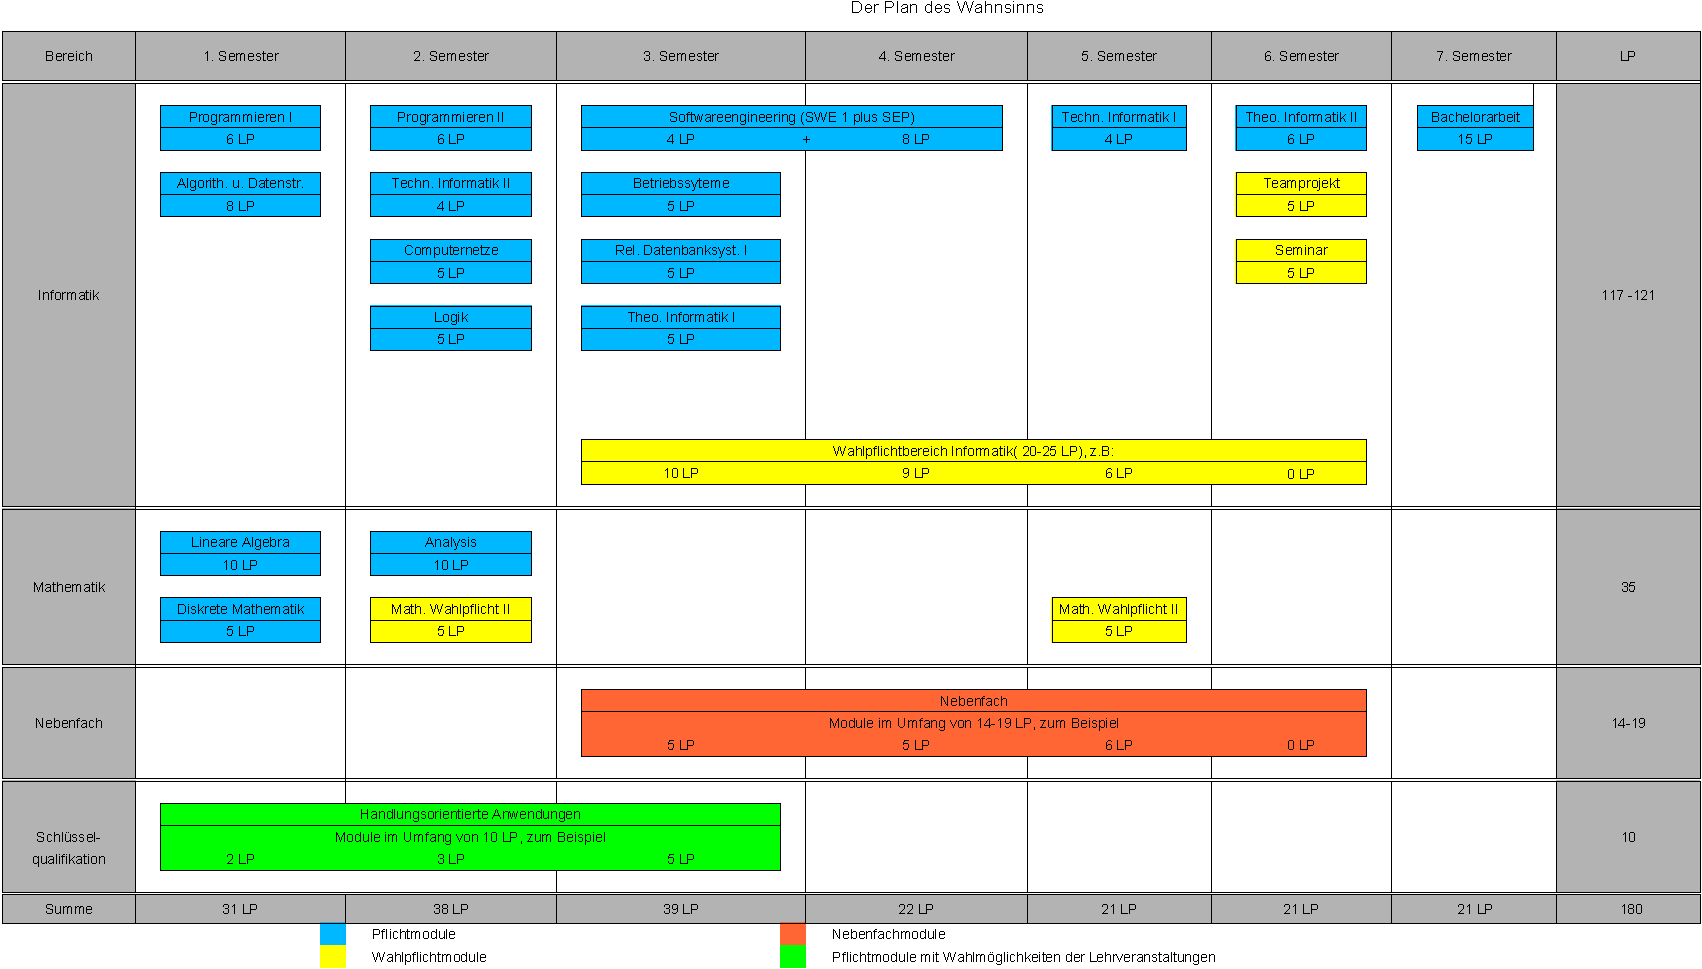
\includegraphics[angle=90,width=\textwidth ]{texte/bachelor/studienplan_joke.pdf}
\end{figure}
\begin{multicols}{2}
% Da ich vom 1. Semester noch ein starkes Interesse für
%Algorithmen hatte
%%% Local Variables: 
%%% mode: latex
%%% TeX-master: "../../1-te"
%%% End: 
